% This template has been downloaded from:
% http://www.latextemplates.com
%
% Original author:
% Ted Pavlic (http://www.tedpavlic.com)
%
% Modified by:
% Charles Newey (http://assemblyco.de)
%----------------------------------------

% Declare document
\documentclass{article}

% Packages
\usepackage{fancyhdr} % Required for custom headers
\usepackage{lastpage} % Required to determine the last page for the footer
\usepackage{extramarks} % Required for headers and footers
\usepackage{graphicx} % Images
\usepackage{tabularx} % Tables
\usepackage[table]{xcolor} % Table colours
\usepackage[colorlinks]{hyperref} % For URLs
\usepackage[T1]{fontenc} % Support symbols like < and >
\usepackage{lmodern} % Format symbols properly

% ToC depth
\setcounter{tocdepth}{6}
\setcounter{secnumdepth}{5}

% Margins
\topmargin=-0.45in
\evensidemargin=0in
\oddsidemargin=0in
\textwidth=6.5in
\textheight=9.0in
\headsep=0.25in
\linespread{1} % Line spacing

% Other setup
\pagestyle{fancy}
\renewcommand\headrulewidth{0.4pt} % Size of the header rule
\renewcommand\footrulewidth{0.4pt} % Size of the footer rule
\setlength\parindent{0pt} % Removes all indentation from paragraphs
\renewcommand{\refname}{} % Removes bibliography title

% Set up constants
\newcommand{\address}{
\small{
	\begin{tabular}{ l}
		Department of Computer Science, \\
		Llandinam Building, \\
		Aberystwyth University, \\
		Aberystwyth, \\
		Ceredigion, \\
		SY23 3DB \\
	\end{tabular}
	}
}

% Set up the header and footer
\lhead{\doctitle}										% Top left header
\chead{\version}										% Top center head
\rhead{\firstxmark \status}								% Top right header
\lfoot{\lastxmark \qanumber}							% Bottom left footer
\cfoot{Aberystwyth University/Computer Science}			% Bottom center footer
\rfoot{Page\ \thepage\ of\ \protect\pageref{LastPage}}	% Bottom right footer

% Set up title page
\title{
	\vspace{1.2in}
	\textmd{\textbf{\doctitle}} \\
	\vspace{0.1in}\large{\textit{\today}} \\
	\vspace{0.4in}
	{\bf{\qanumber}} \\ \vspace{0.4in}
	\version \\
	\status \\
	\vspace{0.4in}
}

\author{\authors}
\date{}


%----------------------------- UPDATE THESE FOR EACH DOCUMENT ------------------------------
\newcommand{\version}{Version: 1.0} %======================================================= DOC VERSION
\newcommand{\status}{Status: Release} %===================================================== DOC STATUS
\newcommand{\qanumber}{SE.10.MAN.1} %=================================================== QA NUMBER
\newcommand{\doctitle}{Group 10 Android Maintenance Manual} %=============================== DOC TITLE

%----------------------------- UPDATE THESE FOR EACH DOCUMENT ------------------------------
%=========================================================================================== VERSION HISTORY
\newcommand{\versionhistory}{
		\begin{tabularx}{\linewidth}{| p{2cm} | p{2cm} | p{2cm} | X | }
			\hline
			\bf{Author} & \bf{Date} & \bf{Version} & \bf{Change made} \\
			\hline
			CCN & 07/11/2013 & 1.0 & Updated order of authors on cover \\
			\hline
		\end{tabularx}
}

%---------------------------- UPDATE THESE FOR EACH DOCUMENT ------------------------------
%=========================================================================================== AUTHOR LIST
\newcommand{\authors}{
	\begin{tabular}{| l | l |}
		\hline
		\bf{Contributor Name} & \bf{Role} \\
		\hline
		Daniel Clark & Project Lead \\
		\hline
		Mark Lewis & QA Manager \& Web Developer \\
		\hline
		Charles Newey & Deputy Project Lead \& Android Developer \\
		\hline
		Martin Ferris & Android Developer \\
		\hline
		Ashley Iles & Android Developer \\
		\hline
		Kenny Packer & Android Developer \\
		\hline
		Stephen McFarlane & Deputy QA \& Web Developer \\
		\hline
		Kieran Palmer & Web Developer \\
		\hline
	\end{tabular}
	% Don't edit this
	\\ \\ \\ \\ \\ \\
	\address \vline
	\hspace{0.15in} \copyright Copyright Group 10, 2014
	% Don't edit this
}

% Make title page, ToC and other introductory elements
\begin{document}
	\maketitle
	\newpage
	\tableofcontents
	\newpage

	% Begin the actual document
	%======================================================================================= DOCUMENT STARTS HERE
	\begin{section}{INTRODUCTION}
		\begin{subsection}{Purpose of This Document}
			To aid with future maintenance of the project's code base, and to document the idiosyncrasies and intricacies of the code used to develop it.
		\end{subsection}
	
		\begin{subsection}{Scope}
			This document should be read by any party that is involved in future maintenance of the application. This document contains details of a number of important factors, including:
			
			{\bf Android}
			\begin{itemize}
				\item{Supported Android SDK versions}
				\item{Main data structures}
				\item{Complex algorithms}
				\item{Suggestions for improvements}
			\end{itemize}
			
			{\bf Website}
			\begin{itemize}
				\item{PHP methods used}
				\item{JavaScript used}
				\item{A basic overview of Google Maps API components used}
				\item{Problematic areas of code}
				\item{Suggestions for improvements}
			\end{itemize}
		\end{subsection}
		
		\begin{subsection}{Objectives}
			\begin{itemize}
				\item{To give an overview into the structure of the application}
				\item{To aid the package maintainer in spotting problem areas in the project's code base}
				\item{To provide the package maintainer a reference for complex areas in the code base}
			\end{itemize}
		\end{subsection}
	\end{section}
	
	\newpage
	
	\begin{section}{Android Maintenance Manual}
	\begin{subsection}{Program information}
		\begin{subsubsection}{Program Description}
			The Stumblr Android application is written in Java and is essentially built to help with the creation and upload of walking tours. It allows the user to record a "breadcrumb trail" of GPS coordinates, and gives the ability to add "Points of Interest" (Waypoints) along the way. The user can attach metadata to each Waypoint - including a title, a description, a photo (from the user's gallery or camera), and a GPS location.  Before uploading, other metadata is attached to the walk - including time taken and cumulative distance. Once the walk is complete, it is then uploaded (in JSON format) to a remote server, where the data is processed and displayed on a web interface.
		\end{subsubsection}
		
		\vspace{0.5in}
		\begin{subsubsection}{Data flow diagram}
			\begin{center}
				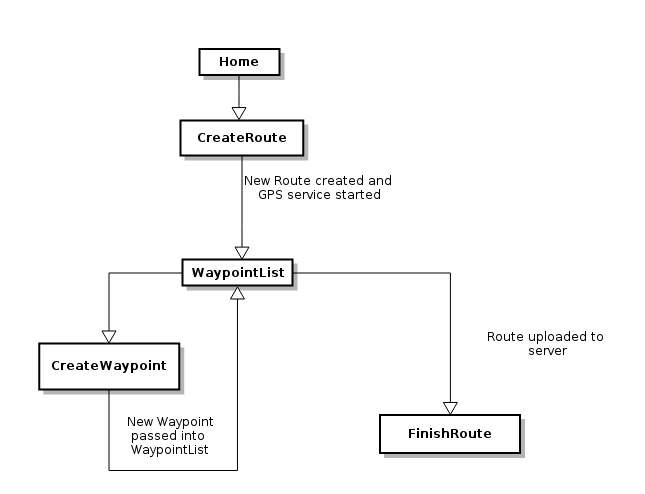
\includegraphics[width=\columnwidth]{img/data_flow}
			\end{center}
		\end{subsubsection}
	\end{subsection}
	
	\newpage
	\begin{subsection}{Data Classes}
		This subsection details the significant or complex methods and data structures in each class - large parts of the code base are very well-commented and self-explanatory, so it is only the more complex areas that are mentioned in this document.
		\begin{subsubsection}{StumblrData}
			\begin{paragraph}{Significant methods}
				\begin{itemize}				
					\item{{\bf public string sanitiseStringInput} \\
					This method takes a String object and replaces all forbidden characters (more specifically, characters that do not belong to the set "a-z", "A-Z", "0-9", ",.!?:;" and "-". This ensures that String data is safe to transmit to the web server.}
				\end{itemize}
			\end{paragraph}
		\end{subsubsection}
	
		\begin{subsubsection}{Route}
			The Route class is the main container for the metadata of the walk - including the description, timestamps, the list of coordinates for the breadcrumb trail, and the list of Waypoints (a datatype that will be covered further later in this document). \\
			
			\begin{paragraph}{Significant data structures}
				\begin{itemize}				
					\item{{\bf private Stack<Location> coordinates;} \\
					This holds the "breadcrumb trail" - a Stack of Location objects (from the Android API). This is where the Location objects are stored when they are obtained from the GPSService class. Location objects are passed from the GPSService class by using Broadcastsm and then filtering by intent. (This is covered in detail later).}
					\item{{\bf private LinkedList<Waypoint> route;} \\
					This holds the list of Waypoint objects - including an instance of a Bitmap image (from the Android API), and Strings relating to the title and description of the Waypoint.}
				\end{itemize}
			\end{paragraph}
			
			\begin{paragraph}{Significant methods}
				\begin{itemize}
					\item{{\bf public float getDistance} \\
					This method calculates the cumulative distance between all of the "breadcrumbs" in the 'coordinates' Stack. The method loops through the list and calls the Android API method {\bf Location.distanceBetween()} on each successive pair of coordinates,. Returns a {\bf float} containing the total distance between each pair of coordinates.}
					
					\item{{\bf public void writeToParcel} \\
					Writes the current contents of the Route object to a {\bf Parcel} object (Android API), to allow the Route to be passed between Activities. Required for implementing the {\bf Parcelable} interface.}
					
					\item{{\bf public void readFromParcel} \\
					Reads a Parcel into the current Route object. Required for implementing the {\bf Parcelable} interface.}
				\end {itemize}
			\end{paragraph}
		\end{subsubsection}
		
		\newpage
		\begin{subsubsection}{Waypoint}
			\begin{paragraph}{Significant methods}
				\begin{itemize}
					\item{{\bf public void writeToParcel} \\
					Writes the current contents of the Waypoint object to a {\bf Parcel} object (Android API), to allow the Route to be passed between Activities. Required for implementing the {\bf Parcelable} interface.}
					
					\item{{\bf public void readFromParcel} \\
					Reads a Parcel into the current Waypoint object. Required for implementing the {\bf Parcelable} interface.}
				\end {itemize}
			\end{paragraph}
		\end{subsubsection}
	\end{subsection}
	
	\begin{subsection}{Activity Classes}
		\begin{subsubsection}{AbstractActivity}
			This class contains all of the common code elements that are used in the other Activities. This includes the code that display the "cancel confirmation" alert dialogue. This class is largely self-explanatory.
		\end{subsubsection}
		
		\begin{subsubsection}{CreateRoute}
			\begin{paragraph}{Significant methods}
				\begin{itemize}
					\item{{\bf public void startWaypointListIntent} \\
					This starts the WaypointList Activity after checking that the input fields of the Activity are the correct length.}
				\end{itemize}
			\end{paragraph}
		\end{subsubsection}
		
		\begin{subsubsection}{CreateWaypoint}
			This Activity is called from the WaypointList activity - and this is where the user can create Waypoints to correspond with Points of Interest (POIs) during the walk.
			\begin{paragraph}{Significant methods}
				\begin{itemize}
					\item{{\bf public void stumblrOnCreate} \\
					This method is essentially the Activity's constructur - it checks the Bundle data passed into the Activity - checking for a Location object or a Waypoint object. The object is then loaded into the appropriate instance variables (depending on the type). The last thing this method does is use the Android API to check if certain capabilities are enabled; namely, a camera and gallery.}
					
					\item{{\bf public void finishWaypoint} \\
					This just validates the data entered on-screen, warning the user with a {\bf Toast} if any data entered is invalid. A timestamp is then applied to the current Waypoint, and the Waypoint object is put into a Bundle as a return value for the Activity - this Bundle is returned to WaypointList (as it is instantiated with {\bf startActivityForResult()}).}
					
					\item{{\bf public void getImage} \\
					Gets an image from user's camera or gallery, after checking which is available. An Activity is dispatched (based upon what is available) using {\bf startActivityForIntent}.}
					
					\item{{\bf protected void onActivityResult} \\
					This method handles return values from the camera or gallery Activities dispatched in the previous method. Depending on the activity that returned the image, it will be resized and cast to a {\bf Bitmap} for easy conversion to Base64, and submission (via JSON) to the web server.}
				\end{itemize}
			\end{paragraph}
		\end{subsubsection}
		
		\newpage
		\begin{subsubsection}{FinishRoute}
		This Activity is responsible for converting the (completed) Route object to JSON and uploading it to the web server, ready for displaying on the web interface. As the data structures dealt with in this class are generally 
			\begin{paragraph}{Significant methods}
				\begin{itemize}
					\item{{\bf public void stumblrOnCreate} \\
					This method is fairly simple - it unbundles the Route object from the extras passed in from the calling Intent, and puts it into memory. The remaining Route metadata is then calculated and displayed onscreen.}
					\item{{\bf public void postData} \\
					This method simply uses the Android API to check if the device has an internet connection - if so, the NetworkTast is executed, and the data is sent.}
					
					\item{{\bf public JSONObject getData} \\
					This converts the Route object into JSON ready for transmission to the web server. This method uses the {\bf JSONObject (org.json.JSONObject)} class from the standard Java JSON libraries.}
					
					\item{{\bf public String encodeToBase64} \\
					This is fairly simple - a {\bf ByteArrayOutputStream} decodes a {\bf Bitmap} object into raw data - which is then encoded using Base64}
				\end{itemize}
			\end{paragraph}
		\end{subsubsection}
		
		\begin{subsubsection}{GPSService}
			GPSService uses a Foreground Notification (to avoid getting killed by Android) and implements {\bf LocationListener} so that it is able to subscribe to Location update (provided by GPS). The {\bf Location} objects are then sent back to the main Activity by using a Broadcast.
			\begin{paragraph}{Significant methods}
				\begin{itemize}
					\item{{\bf public int onStartCommand} \\
					This is a rather straightforward method, but it looks a little complicated. It subscribes the current class to receive {\bf Location} updates and places a persistent {\bf Notification} in the user's Notification Centre. {\bf Be aware: There is officially deprecated code inside this method so that the persistent Notification can be shown on older versions of Android.}}
					\item{{\bf public void onDestroy} \\
					This method tells the class to stop receiving Location updates when killed - this ensures that the device's battery is not wasted.}
					\item{{\bf public void onLocationChanged} \\
					This method is very simple, but its function may not be immediately obvious. It is called when a {\bf Location} update is received by the {\bf GPSService} class, and it bundles the received {\bf Location} object and sends it as a {\bf Broadcast} to the system, where the message is picked up by {\bf WaypointList} and added to the current Waypoint.}
				\end{itemize}			
			\end{paragraph}
		\end{subsubsection}
		
		\begin{subsubsection}{Home}
			The Home class contains no complex methods as it is approximately 35 lines in length and only contains code for one button!
		\end{subsubsection}
		
		\newpage
		\begin{subsubsection}{WaypointList}
			This is the main Activity of the application in that most of the user's time is spent using it. From this Activity, the user can view, add to, and edit the current list of Waypoints. The user can also decide to complete the walk, dispatching the FinishRoute Activity.
			\begin{paragraph}{Significant data structures}
				\begin{itemize}
					\item{{\bf private ListView listView} \\
					This ListView object is used to display and manipulate the Route's Waypoints on-screen. The user can view a list of the current Waypoints, or edit the}
				\end{itemize}
			\end{paragraph}
			
			
			\begin{paragraph}{Significant methods}
				\begin{itemize}
					\item{{\bf protected void onActivityResult} \\
					This method is called when a dispatched Activity (in this case, CreateWaypoint) exits and returns with a valid Waypoint object - the new Waypoint is added to the list and the ListView is refreshed.}
					
					\item{{\bf private void startGPSService} \\
					There is a private class declaration within this method that contains methods to add coordinates received from the GPSService to the current trail of {\bf Locations}. If GPS is disabled, the method prompts the user to enable it.}
					
					\item{{\bf public void onDestroy} \\
					Called before the Activity is destroyed (part of the Android application lifecycle). This sends a signal to the running GPS service to halt and exit (thus removing the {\bf Notification} at the top of the user's screen).}
				\end{itemize}
			\end{paragraph}
		\end{subsubsection}
	\end{subsection}
	
	\begin{subsection}{Limitations of the Application}
		There are a number of limitations to the application in question, the principal of which are the Android API versions that it supports. Currently, the application supports (and has been fully tested on) API/SDK versions {\bf 8} to {\bf 22} - which correlates to Android versions {\bf 2.2} through {\bf 4.4}. \\
		
		There are also a number of important considerations when it comes to battery and memory usage. Each Waypoint (including thumbnail image) is stored entirely in working memory (RAM) - theoretically, this limits the number of Waypoints that a low-RAM device can hold; although in practice, the amount of data in memory (even on large walks) is relatively small, and memory usage is a very minor consideration. Certainly, we experienced no issues on an older Android {\bf 2.3} device with severe memory limitations, with walks of 20 Waypoints and above. \\
		
		The application is also rather battery intensive on longer walks; the GPS service, while being useful for regularly fetching location data - uses an enormous amount of battery power, particularly if the GPS signal is bad (due to overcast weather, large buildings in the surrounding area, etc). This is sufficient to flatten some more power-hungry devices with 5-6 hours' usage (tested overnight on a tablet device).
	\end{subsection}
	
	\begin{subsection}{Interaction with Remote Server}
		The interaction with the server is kept as simple as possible. The Java objects created within the application are converted to JSON (a human-readable format useful when transmitting complex objects), and transferred to the server via HTTP POST. The HTTP interaction is completed with the Apache Commons HTTP libraries, and the code used to interact with the server is currently in the FinishRoute class.
	\end{subsection}
	
	\newpage
	\begin{subsection}{Building and Testing}
		This subsection details the tools and methods that were used to create and compile the application and documentation.
		
		\begin{subsubsection}{Building}
			The build tools used in the creation of the Java code base were Android Studio, coupled with the Gradle build system. The supplementary files inside the Git repository are mostly to ensure proper functioning of Gradle and the Android Studio IDE.
		\end{subsubsection}
		
		\begin{subsubsection}{Testing}
			The testing code for this assignment was written using JUnit - a testing suite that complements the Java language.
		\end{subsubsection}
		
		\begin{subsubsection}{Documentation}
			All documentation for this project (where possible) has been written and rendered using \LaTeX. \LaTeX can be a challenge to write for new users, so a procedure was defined for team members who struggle getting it to work; writing documents in MarkDown and then converting them. MarkDown is a minimal, intuitive markup language (also used on GitHub for formatting text files) that aims to be easy to write. This was excellent for our needs, as MarkDown syntax can be easily converted to \LaTeX syntax using a system like PanDoc. \\ \\
			Markdown: \url{https://daringfireball.net/projects/markdown/} \\
			PanDoc: \url{http://johnmacfarlane.net/pandoc/}
		\end{subsubsection}
		
		\begin{subsubsection}{References to external sources}
			References to external sources are usually contained inside inline comments in the Java code; {\em for example}: \\ \\
			{\tt // See: somewebsite.com/url/resource.html}
		\end{subsubsection}
	\end{subsection}
	\end{section}
	
	\begin{section}{Website Maintenance Manual}
		\subsection{Website Description}
		This website is a walking tour viewer, it pulls data from a database which is provided by the android application Stumblr. It then uses this data in conjunction with the Google maps API on the website to display the tour on the map, including information on the locations visited on the route. It also provides a gallery bar of all the images of the tour selected if there are any.
		
		The system uses a database to store details on the tours captured using the Android app. The details stored in the database are then displayed on the website using a combination of SQL commands and PHP scripts. The database itself contains three tables, all storing different information on the tours. The tables store information on each walk, their location and also the path for each walk. 

		\subsection{Website Structure}
		I will show the structure of this website in two ways; first I will provide you with the flow of the website to show you how it works then, I will go through the code saying what the methods and sections of the code do.

		There are four main components to the websites; HTML, JavaScript, PHP and the database. All of  these all work together to create the web page Stumblr. 

		\subsubsection{HTML}
The HTML is what I have used for the design such as having the body of the web page centred using a div called divwrapper which has been set to be 80\% width of the browser screen. The HTML includes the divs tour, map and bar. The tour div is where information of the tour is presented when the tour is loaded this will contain the name and description of the tour plus any other information held in the database. The map div is used to hold the Google map which is created by the JavaScript this is set to the width of the body. The bar div is where the gallery of images is shown as a scrollable list of images with their title and description. The HTML also has the form which is used to select and load a tour which it does by sending the ID of the tour back to the page using POST. It gets the ID and title of the tour in this from by using php to get the information from the database.

		\subsubsection{JavaScript}
		The JavaScript is used to create the map and gather information from the database to populate that map. The JavaScript in this web page has 3 functions downloadUrl(), bindfInfoWindow() and load() which I will talk about now :

downloadUrl() - this function is just a basic download function to download a url, in this case we are using it to download an XML file. The XML file contains all the details of the selected tour. 

load() - this function loads up the google map, by default it displays nothing as no tour is selected. If a tour is selected it will display on the map. First it creates a variable called map which is a new Google map, the next few variables are first where the map should be centred which is the co-ordinates of the centre of Aberystwyth town, next is the zoom level of the map which controls the level of zoom on the co-ordinates and the last one is the map type which is roadmap so people can see the roads and also use Google street-view. Next the downloadUrl() function is called to download XMLcreator.php. This contains the details of the tour. Next the variable markers are created by getting information from the XML document. A loop is used to set the variables for information to be displayed as a marker, below is the code for a marker:

\begin{verbatim}
var marker = new google.maps.Marker({map: map, position: point,
icon: "images/mapiconscollection-numbers-fa0505-classic/number_" + i + ".png"});
bindInfoWindow(marker, map, infoWindow, html);
\end{verbatim}

Then info window is also added here using the information from the tour as you can above.

		The next part is where the function downloads the xmlpath.php file that is used to create a route between the markers on the map. This works a little like the inner function that creates the markers and info windows as it uses a variable paths instead of markers but this function also uses a variable pathco which is an array to hold all the co-ordinates of the path to be used later. The loop gets the length of the route from the XML file, it then gets the co-ordinates of the route taken and sets them to a variable called point. This variable is then pushed to the pathco variable using the following code:    pathco.push(point);    this is used to push all the variables to this array to create an array of the path co-ordinates. Below this you will see the path options being set such as the path variable being set to the pathco array, and other options such as strokeColor, opacity and weight which can be altered to create a different route look, then below the path is set to the map.

bindInfoWindow() -  This function is used to tie all the markers and infoboxes to the map and where a listener is added that when markers have been clicked  they open an infobox with the information in the html variable.

		\subsubsection{PHP}
		The PHP used in this website is mostly used to get information from the database but there are a few lines that are used for other things. \\

		At the top of the page you will see: session\_save\_path(); session\_start(); \\
This is used to set where sessions will be saved to a tmp folder as most web servers will save sessions to a tmp folder if the path is an empty string. Then it starts off the session using the session\_start().

		Then the variable \$walkID is created and set to zero so when first opened the web page will come up with a default map instead of a tour. Then if somebody loads up a tour it will send a POST back to the page which is why the next line is the variable being set to \$\_POST['tours'] so \$walkID will be equal to the tour that has been selected. Then a session variable is created which is also equal to the POST which is used in the XML files to get the correct tour for the Google map. \\

		Then the next few lines are used to connect to the database and then query tables in that database to get information which is to be used on the webpage. Next there is an IF statement just encase there are problems connecting to the server, including the error message "Failed to connect to MySQL: ".
PHP is next used to create a drop down box that contains the names of all the tours on the database, it uses a query that is created at the top of the page to get the information from the database.
Then the information about the tour that is loaded tis display above the map. This includes the tour's title, long description, short description, time and distance.
Finally there is the gallery where we use the same query used above to display the images for each tour. The image is base64 encoded and must be decoded before being displayed. It is displayed along with a title and description.

		\subsubsection{Database}
		The first table is used to store the walks, it holds information on the title stored as a varchar, short description stored as a varchar , long description stored as a varchar, time taken stored as a float and distance also as a float. The primary key is used to reference the other details of each tour in the other tables. The next table used contains details on each location for a walk. The table stores each locations title, short description, long description all as a varchar, longitude, latitude and a time stamp as a float and finally an image stored as long text due to the images being base 64 encoded.. The table also has an ID as a primary key, as well as a foreign key which links the location to a walk in the walks table.
The final table used in the database stores a path for each walk. Therefore it has a foreign key integer which references to the walk it represents, a value for the longitude and latitude which are both stored as floats. 


		\subsubsection{Algorithms}
		The main algorithm used for this webpage is creating an XML file of information from the database. This is used in both XMLcreator.php and xmlpath.php . They do this by connecting to the database, and then pulling data from the table that the information is in. Next it iterates through the rows adding XML nodes for each part, which is then used in index.php when the function downloadUrl() is called to get this information which it loops through to get all of the information.


		\subsubsection{Files}
		For the website there is an extra file the Cascading Style Sheet, which is used for the design of the page such as the background and how big the body of the website is going to be and also all the sizes of the divs.

		In order to access the data in the database three files containing PHP scripts were used. Two of the files where used for converting the data into XML, one for the locations on a tour and another for the path. Then the XML could be used to display the tours in conjunction with Google Maps. The way these scripts work is to first connect to the database, then they use SQL queries to find which data in the database they need depending on which tour is selected. Finally they pull the data from the database and insert it into a new XML file. The final file which is used is another PHP script and this decodes the incoming data in the form of a JSON file and inserts them into the database. Firstly the script establishes a connection to the database, then it takes in the JSON file and decodes it using a PHP function called json\_decode. Next it stores the decoded data as variables and these variables are using along with SQL commands to add the data to the database. 

		\subsubsection{Interfaces}
		The main interface with the website is the Google map which I have gone over in some length in the website structure above. If you wanted to know more about this interface then there is a Google Maps API. The only other interface with this website is the drop down box and load tour button which is generated with some PHP and they are located in a form which sends the id of the tour back to the page so it loads that tour up from the database.

		\subsubsection{Suggestions for Improvements}
		A few improvements I could suggest would be to improve the look of the gallery bar at the bottom of the page so the titles, pictures and description line up properly, this probably be done with some new divs in the CSS file. Another improvement I could suggest  is the way information about the tour is loaded above the map which could be done with several little things such as a border or the changes to the div and how the information it presented with the <p> tags. Another suggestion would be the background of the web-page as I have seen it tile at the bottom when there is to much information on the page that it makes it tile this could probably be fixed by changing the CSS for the background or you could get a bigger picture.
		Another suggestion for improvement would be to add PHP unit tests to website as they are none right now, it would be good to have these so if something goes wrong you will know were the problem is.


		\subsubsection{Things to Watch When Making Changes}
		There are many things to watch for when making changes I will now go through some with the website and the database.
		Website

		The thing you most want to watch out for when making changes to the website is the JavaScript as one small change and a whole bunch of problems can happen. I would recommend having a backup of the file working before making changes to see where you might have gone wrong. Another way you could prevent from getting errors with the Google maps JavaScript is to go through their website as they have many example of a working Google map. Also another thing to watch out for when making changes to the website is that you use the right queries for getting information out of the database. Also when testing the website if would use the browsers debugger like Firefox’s this can tell you were you are going wrong.

		\subsubsection{Database}
		Changing the overall structure of the database will have knock on effects on the rest of the system. Most of the PHP code used for accessing the database uses variables and statements which rely on the names of columns in the database. The areas that it would affect would include pulling data, decoding the JSON and inserting data into the database. Therefore it is important that if any changes are made to the database they are made to every PHP file. 

		\subsubsection{Physical limitations of the program}
		A physical limitations of our website is that the database is held on a different database to the website which means if it goes down there is now way of using the information on the database with the website. This means if it went down the website would not be able to get any information for the tour leaving it mostly blank and useless.


		\subsubsection{Rebuilding and testing}
			There is no need for rebuilding of the website as PHP is an interpreted language so it does not need to be rebuilt.
	
			For testing there are not PHP unit tests in the website so you can only browser test it to make sure that it works on the most popular browsers.
	\end{section}
	
	\begin{section}{Database Maintenance Manual}
		\subsection{Description}
		The system use a database to store details on the tours captured using the android app. The details stored in the database are then displayed on the website using a combination of SQL commands and PHP scripts. The database itself contains three tables, all storing different information on the tours. The tables store information on each walk, their location and also the path for each walk.


		\subsection{Structure}
		The first table is used to store the walks, it holds information on the title stored as a varchar, short description stored as a varchar , long description stored as a varchar, time taken stored as a float and distance also as a float. The primary key is used to reference the other details of each tour in the other tables. \\
		
		The next table used contains details on each location for a walk. The table stores each locations title, short description, long description all as a varchar, longitude, latitude and a time stamp as a float and finally an image stored as long text due to the images being base 64 encoded.. The table also has an ID as a primary key, as well as a foreign key which links the location to a walk in the walks table. \\
		
		The final table used in the database stores a path for each walk. Therefore it has a foreign key integer which references to the walk it represents, a value for the longitude and latitude which are both stored as floats. 

		\subsection{Files}
		In order to access the data in the database three files containing PHP scripts were used. Two of the files where used for converting the data into XML, one for the locations on a tour and another for the path. Then the XML could be used to display the tours in conjunction with Google Maps. The way these scripts work is to first connect to the database, then they use SQL queries to find which data in the database they need depending on which tour is selected. Finally they pull the data from the database and insert it into a new XML file. \\
		
		The final file which is used is another PHP script and this decodes the incoming data in the form of a JSON file and inserts them into the database. Firstly the script establishes a connection to the database, then it takes in the JSON file and decodes it using a PHP function called json\_decode. Next it stores the decoded data as variables and these variables are using along with SQL commands to add the data to the database.

		\subsection{Things to Watch When Making Changes}
		Changing the overall structure of the database will have knock on effects on the rest of the system. Most of the PHP code used for accessing the database uses variables and statements which rely on the names of columns in the database. The areas that it would affect would include pulling data, decoding the JSON and inserting data into the database. Therefore it is important that if any changes are made to the database they are made to every PHP file.
	\end{section}
	
	% Include references here (edit the References.bib file)
	\nocite{LaTeXTemplate} % DO NOT EDIT

	% Format bibliography/refs
	\newpage
	\begin{section}{REFERENCES}
		\bibliographystyle{acm}
		\bibliography{References}
	\end{section}
	
	\vspace{1cm}
	\begin{section}{VERSION HISTORY}
		\versionhistory
	\end{section}
\end{document}

%									Useful bits and pieces
%\begin{subsection}{subsection_name}								% Start subsection
%\end{subsection}												% End subsection
%\begin{center} \end{center}								% Center stuff
%\includegraphics[width=0.75\columnwidth]{example_figure}	% Insert image
%\pseudocode{filename}{caption}								% Insert highlighted code snippet
%\clearpage													% Clear page after subsection
%\url{http://www.google.com/} 								% Include URL
%\nocite{citationName}										% Cite to bibliography (but not to text)
%\cite{citationName}										% Include reference